% In \textbf{Graph}, pullbacks and pushouts always exist. A pushout of a span of monomorphisms and a pullback of a cospan of monomorphisms are easy to construct: at the cost of graph renaming, a pushout can be constructed by setting the pushout graph as the union of graphs and the cospan as a pair of subgraph embeddings; Similarly, a pullback  can be constructed by setting the pullback graph as the intersection of graphs and the span as a pair of subgraph embeddings.
% In the category \(\mathbf{Graph}\), pullbacks and pushouts always exist. Constructing them is straightforward when dealing with monomorphisms (injective homomorphisms), because, with possibly renaming of nodes, a span with injective homomorphisms has the form of \( A \uplus B' \overset{\alpha}{\leftarrowtail} A \overset{\beta}{\rightarrowtail} A \uplus C' \), therefore a pushout is \( A \uplus B' \overset{\alpha}{\rightarrowtail} A \uplus B' \uplus C' \overset{\beta}{\leftarrowtail} A \uplus C' \). Similarly, a cospan with injective homomorphisms has,  with possibly renaming of nodes,  the form of \( A \uplus B' \overset{\alpha}{\rightarrowtail} A \uplus B' \uplus C' \overset{\beta}{\leftarrowtail} A \uplus C' \), hence a pullback is \( A \uplus B' \overset{\alpha}{\leftarrowtail} A \overset{\beta}{\rightarrowtail} A \uplus C' \). They share the same diagram depicted below:

% \begin{center}
%     \begin{tikzpicture}
%                 \node (i) at (0,0) {A};
%                 \node (r) at (2,1) {$A \uplus B'$};
%                 \node (c) at (2,-1) {$A \uplus C'$};
%                 \node (h) at (4,0) {$A \uplus B' \uplus C'$};
%                 \draw[>->]  (i) -- (r) node [midway,left] { };
%                 \draw[>->] (c) -- (h) node [midway,left] { };
%                 \draw[>->] (r) -- (h) node[midway, left] { };
%                 \draw[>->] (i) -- (c) node[midway, left] { };
%             \end{tikzpicture}
% \end{center}

%  For a pushout of a span \( B \overset{\alpha}{\leftarrowtail} A \overset{\beta}{\rightarrowtail} C \) of injective homomorphisms, we first rename vertices of $B$ and $C$ to obtain the span \( A \uplus B' \overset{i}{\leftarrowtail} A \overset{j}{\rightarrowtail} A \uplus C' \) where $i, j$ are inclusion function, then \( B \overset{\alpha}{\rightarrow} A \overset{\beta}{\rightarrowtail} C \) create the pushout graph by taking the union of the graphs, renaming vertices if necessary to avoid conflicts. This results in a cospan of subgraph embeddings into the pushout graph. Similarly, for a pullback of two graphs connected by monomorphisms, we form the pullback graph by taking the intersection of the graphs, accompanied by a span of subgraph embeddings from the pullback graph to the original graphs.


% In the category \(\mathbf{Graph}\), pullbacks and pushouts always exist, and their construction is straightforward when dealing with monomorphisms (injective graph homomorphisms). 
% Let $\uplus$ denote the disjoint union operation. For two sets \(A\) and \(B\), their disjoint union \(A \uplus B\) is defined as the set of ordered pairs \( (x, i) \) where \( x \mathop{\in} A \) if \( i \mathop{=} 1 \) and \( x \mathop{\in} B \) if \( i \mathop{=} 2 \). Formally, we have:
% $
% A \uplus B \mathop{=} \{ (x, 1) : x \mathop{\in} A \} \mathop{\cup} \{ (x, 2) : x \mathop{\in} B \}.
% $ 
% By possibly renaming nodes, a span of injective graph homomorphisms can be represented as
% $
% A \uplus B' \overset{\alpha}{\leftarrowtail} A \overset{\beta}{\rightarrowtail} A \uplus C'.
% $
% where $\alpha$ and $\beta$ are inclusion function. A pushout of this span is then given by
% $
% A \uplus B'  \overset{\beta'}{\rightarrowtail} A \uplus B' \uplus C'   \overset{\alpha'}{\leftarrowtail} A \uplus C'
% $ where $\alpha'$ and $\beta'$ are inclusion function.
% Similarly, a cospan of injective graph homomorphisms, possibly with renamed nodes, takes the form
% $
% A \uplus B'  \overset{\beta'}{\rightarrowtail} A \uplus B' \uplus C'   \overset{\alpha'}{\leftarrowtail} A \uplus C'
% $ where $\alpha'$ and $\beta'$ are inclusion function.
% and a pullback is
% $
% A \uplus B' \overset{\alpha}{\leftarrowtail} A \overset{\beta}{\rightarrowtail} A \uplus C'.
% $ where $\alpha$ and $\beta$ are inclusion function.
% Both constructions share the same underlying commutative diagram, where the monomorphisms are inclusion functions. This diagram is depicted below:
In the category \(\mathbf{Graph}\), pullbacks always exist, and their construction is straightforward when dealing with monomorphisms (injective graph homomorphisms). 
% Let $\uplus$ denote the disjoint union operation. For two sets \(A\) and \(B\), their disjoint union \(A \uplus B\) is defined as the set of ordered pairs \( (x, i) \) where \( x \mathop{\in} A \) if \( i \mathop{=} 1 \) and \( x \mathop{\in} B \) if \( i \mathop{=} 2 \). Formally, we have:
% $
% A \uplus B \mathop{=} \{ (x, 1) : x \mathop{\in} A \} \mathop{\cup} \{ (x, 2) : x \mathop{\in} B \}.
% $ 
We denote $X\uplus Y$ the union of two disjoint sets. 
Similarly, a cospan of injective graph homomorphisms, possibly with renamed nodes, takes the form
$
A \uplus B'  \overset{\beta'}{\rightarrowtail} A \uplus B' \uplus C'   \overset{\alpha'}{\leftarrowtail} A \uplus C'
$ where $A, B', C'$ are disjoint sets and $\alpha', \beta'$ are inclusion function. A pullback of this cospan is
$
A \uplus B' \overset{\alpha}{\leftarrowtail} A \overset{\beta}{\rightarrowtail} A \uplus C'
$ where $\alpha$ and $\beta$ are inclusion function.
The diagram is depicted below:

\begin{figure}[htbp] 
    \center
    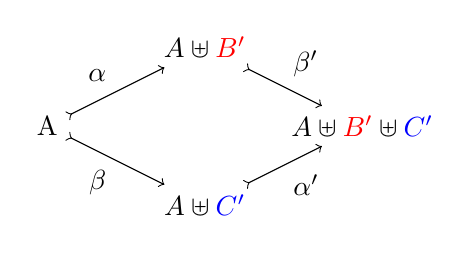
\begin{tikzpicture}
        \node (i) at (0,0) {A};
        \node (r) at (2,1) {$A \uplus \textcolor{red}{B'}$};
        \node (c) at (2,-1) {$A \uplus \textcolor{blue}{C'}$};
        \node (h) at (4,0) {$A \uplus \textcolor{red}{B'} \uplus \textcolor{blue}{C'}$};
        \draw[>->]  (i) -- (r) node [midway, above left] {$\alpha$};
        \draw[>->] (c) -- (h) node [midway, below right] {$\alpha'$};
        \draw[>->] (r) -- (h) node[midway, above right] {$\beta'$};
        \draw[>->] (i) -- (c) node[midway, below left] {$\beta$};
\end{tikzpicture}
    \caption{}
    \label{fig:pb_decomp}
\end{figure}

\begin{example}
    \label{ex:pb_in_graph}
    The diagram in Figure~\ref{fig:ex:pb_in_graph} is a pullback square in the category \textbf{Graph} where nodes and arrows are colored to visualize the decomposition as in Figure~\ref{fig:pb_decomp}.
    
\begin{figure}[H] 
    \center
    \begin{center}
    \resizebox{0.4\textwidth}{!}{
        \begin{tikzpicture}
               
                \graphbox{ }{40mm}{5mm}{34mm}{15mm}{2mm}{0mm}{
                    \coordinate (o) at (0mm,-8mm); 
                    \node[draw,circle] (l1) at ($(o)+(-10mm,0mm)$) {1};
                    \node[draw,circle] (l2) at ($(l1)+(2,0)$) {2};
                }  
  
                \graphbox{ }{80mm}{5mm}{45mm}{15mm}{2mm}{-0mm}{
                    \coordinate (o) at (-5mm,-8mm); 
                    \node[draw,circle] (l1) at ($(o)+(-10mm,0mm)$) {1};
                    \node[draw,circle] (l2) at ($(l1)+(3,0)$) {2};
                    \node[red,draw,circle] (l3) at ($(l1)+(1,0)$) {4};
                    \node[red,draw,circle] (l4) at ($(l1)+(2,0)$) {5};
                    \draw[red] (l1) -- (l3) node[midway,above] {$a$};
                    \draw[red] (l3) -- (l4) node[midway,above] {$b$};
                    \draw[red] (l4) -- (l2) node[midway,above] {$a$};
                }    
                \graphbox{ }{40mm}{-17mm}{34mm}{25mm}{2mm}{-5mm}{
                    \coordinate (o) at (0mm,-3mm); 
                    \node[draw,circle] (l1) at ($(o)+(-10mm,0mm)$) {1};
                    \node[draw,circle] (l2) at ($(l1)+(2,0)$) {2};
                    \node[blue,draw,circle] (l4) at ($(l2)+(0,-1)$) {6};
                    \draw[blue] (l2) -- (l4) node[midway,right] {$a$};
                    \node[blue,draw,circle] (l6) at ($(l1)+(0,-1)$) {7};
                    \draw[blue] (l1) -- (l6) node[midway,left] {$a$};
                }    
  
                \graphbox{ }{80mm}{-17mm}{45mm}{25mm}{2mm}{-5mm}{
                    \coordinate (o) at (-5mm,-3mm); 
                    \node[draw,circle] (l1) at ($(o)+(-10mm,0mm)$) {1};
                    \node[draw,circle] (l2) at ($(l1)+(3,0)$) {2};
                    \node[draw,circle,red] (l3) at ($(l1)+(1,0)$) {4};
                    \node[draw,circle,red] (l4) at ($(l1)+(2,0)$) {5};
                    \node[blue,draw,circle] (l5) at ($(l2)+(0,-1)$) {6};
                    \node[blue,draw,circle] (l6) at ($(l1)+(0,-1)$) {7};
                    \draw[blue] (l1) -- (l6) node[midway,left] {$a$};
                    \draw[red] (l1) -- (l3) node[midway,above] {$a$};
                    \draw[red] (l3) -- (l4) node[midway,above] {$b$};
                    \draw[red] (l4) -- (l2) node[midway,above] {$a$};
                    \draw[blue] (l2) -- (l5) node[midway,right] {$a$};
                }    
  
                \node () at (77mm,-3mm) {\( \rightarrowtail \)}; % K -> R
                \node () at (52mm,-13mm) {\( \downarrowtail \)};
                \node () at (92mm,-13mm) {\( \downarrowtail \)};
                \node () at (77mm,-28mm) {\( \rightarrowtail \)}; % C -> H
        \end{tikzpicture}
    }
\end{center}
\caption{Example of the pullback of cospan of monomorphism in \(\mathbf{Graph}\)}
\label{fig:ex:pb_in_graph}
\end{figure}
\end{example}

The compositions \( \beta' \circ \alpha \) and \( \alpha' \circ \beta \) both map elements from \( A \) to \( A \uplus B' \uplus C' \) via inclusion function.
Since all maps are inclusions and \( A \), \( B' \), and \( C' \) are disjoint, the square commutes $
     \beta' \circ \alpha \mathop{=} \alpha' \circ \beta 
$. 

To demonstrate that Figure~\ref{fig:pb_decomp} is a pullback square, suppose we have an object \( X \) and morphisms \( f: X \mathop{\to} A \uplus B' \) and \( g: X \mathop{\to} A \uplus C' \) such that
$
\alpha' \circ f \mathop{=} \beta' \circ g.
$
Our goal is to prove that there exists a unique morphism \( h: X \mathop{\to} A \) such that
$
\alpha \circ h \mathop{=} f \quad \text{and} \quad \beta \circ h \mathop{=} g.
$

Since \( \alpha' \) and \( \beta' \) are inclusion maps into \( A \uplus B' \uplus C' \), and \( \alpha' \circ f \mathop{=} \beta' \circ g \), it follows that for all \( x \mathop{\in} X \),
$
f(x) \mathop{=} g(x) \mathop{\in} A \uplus B' \uplus C'.
$
Because \( B' \) and \( C' \) are disjoint and their images under \( \alpha' \) and \( \beta' \) are also disjoint in \( A \uplus B' \uplus C' \), the only way \( \alpha' \circ f(x) \mathop{=} \beta' \circ g(x) \) is if both \( f(x) \) and \( g(x) \) are in \( A \) and map to the same element in \( A \uplus B' \uplus C' \).
Therefore, \( f(x), g(x) \mathop{\in} A \) and \( f(x) \mathop{=} g(x) \).
We can now define \( h: X \mathop{\to} A \) by
$
h(x) \mathop{=} f(x) \mathop{=} g(x) \quad \text{for all } x \mathop{\in} X.
$


We need to verify that
$
\alpha \circ h \mathop{=} f \quad \text{and} \quad \beta \circ h \mathop{=} g.
$
Since \( \alpha \) and \( \beta \) are inclusion maps of \( A \) into \( A \uplus B' \) and \( A \uplus C' \), respectively, it follows that
$
\alpha \circ h(x) \mathop{=} \alpha(f(x)) \mathop{=} f(x), \quad \text{since } h(x) \mathop{=} f(x) \text{ and } \alpha \text{ is inclusion}.
$
Similarly,
$
\beta \circ h(x) \mathop{=} \beta(g(x)) \mathop{=} g(x).
$

Suppose there exists another morphism \( h': X \mathop{\to} A \) satisfying \( \alpha \circ h' \mathop{=} f \) and \( \beta \circ h' \mathop{=} g \). Then for all \( x \mathop{\in} X \),
$
f(x) \mathop{=} \alpha \circ h'(x), \quad g(x) \mathop{=} \beta \circ h'(x).
$
Since \( \alpha \) and \( \beta \) are inclusions, \( \alpha \circ h'(x) \mathop{=} h'(x) \) in \( A \uplus B' \) and \( \beta \circ h'(x) \mathop{=} h'(x) \) in \( A \uplus C' \). Therefore,
$
f(x) \mathop{=} h'(x) \mathop{=} g(x).
$
But we already have \( h(x) \mathop{=} f(x) \mathop{=} g(x) \), so \( h'(x) \mathop{=} h(x) \) for all \( x \mathop{\in} X \). Thus, \( h \) is unique.

Since there exists a unique morphism \( h: X \mathop{\to} A \) such that \( \alpha \circ h \mathop{=} f \) and \( \beta \circ h \mathop{=} g \), the diagram in Figure~\ref{fig:pb_decomp} satisfies the universal property of the pullback. Therefore, the diagram is indeed a pullback square.